\documentclass[10pt]{exam}
\usepackage[hon]{template-for-exam}
\usepackage{endnotes,graphicx}
\usepackage{tikz,graphicx,enumitem,multicol,float,my-tikz-clipart,silence,cclicenses}
\graphicspath{{./figures/}}
\WarningFilter{latex}{Label `part}
\WarningFilter{latex}{There were multiply-defined labels}
\usetikzlibrary{arrows.meta}

\footer{}{\thepage}{\sc \myclass}


%\def\answer#1{\footnotetext{#1}}
%\def\myquestion{\item\stepcounter{footnote}}

\def\enoteheading{}
\def\answer#1{\endnotetext{#1}}
\def\theanswers{\theendnotes}
\def\myquestion{\item\stepcounter{endnote}}

\newenvironment{myquestions}{
  \begin{multicols}{2}\begin{enumerate}[resume]
}{
  \end{enumerate}\end{multicols}
}
\makeatletter
\patchcmd{\enit@setresumekeys}{\def}{\gdef}{}{}
\patchcmd{\enit@setresumekeys}{\def}{\gdef}{}{}
\makeatother

\newcommand{\myheading}[1]{\uplevel{\section*{#1}}
}
\newcommand{\mysubheading}[1]{\uplevel{\subsection*{#1}}
}

%uncomment if running Pandoc
% \renewcommand{\myheading}[1]{{\section*{#1}}}
% \renewcommand{\mysubheading}[1]{\subsection*{#1}}

\title{Chapter 3 Homework A (Vectors in 2D)}
\author{Rohrbach}
\date{\today}

\def\mymaketitle{
  \begin{flushleft}
    {\LARGE \textbf \mytitle \par}
  \end{flushleft}
}

\newcommand{\bs}[2]{\textbf{#1} (\sc #2 Points)}


\newcommand{\GFig}[2]{  
  \begin{figure}[H]
    \centering
    \includegraphics[width=#2]{11_#1_Figure.jpg}
    \caption{Giancolli Figure 11-#1.}
    \label{11-#1}
  \end{figure}
}


\begin{document}
\maketitle


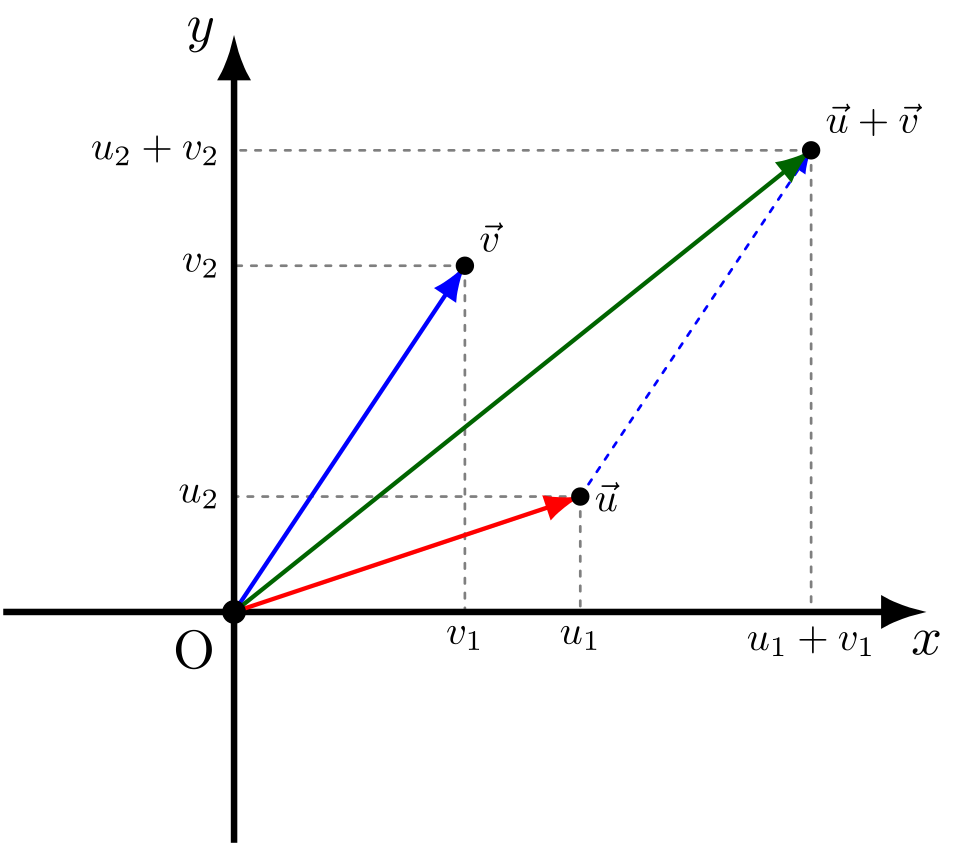
\includegraphics[height=2.5in]{vectors.png}
%
\hfill 
%
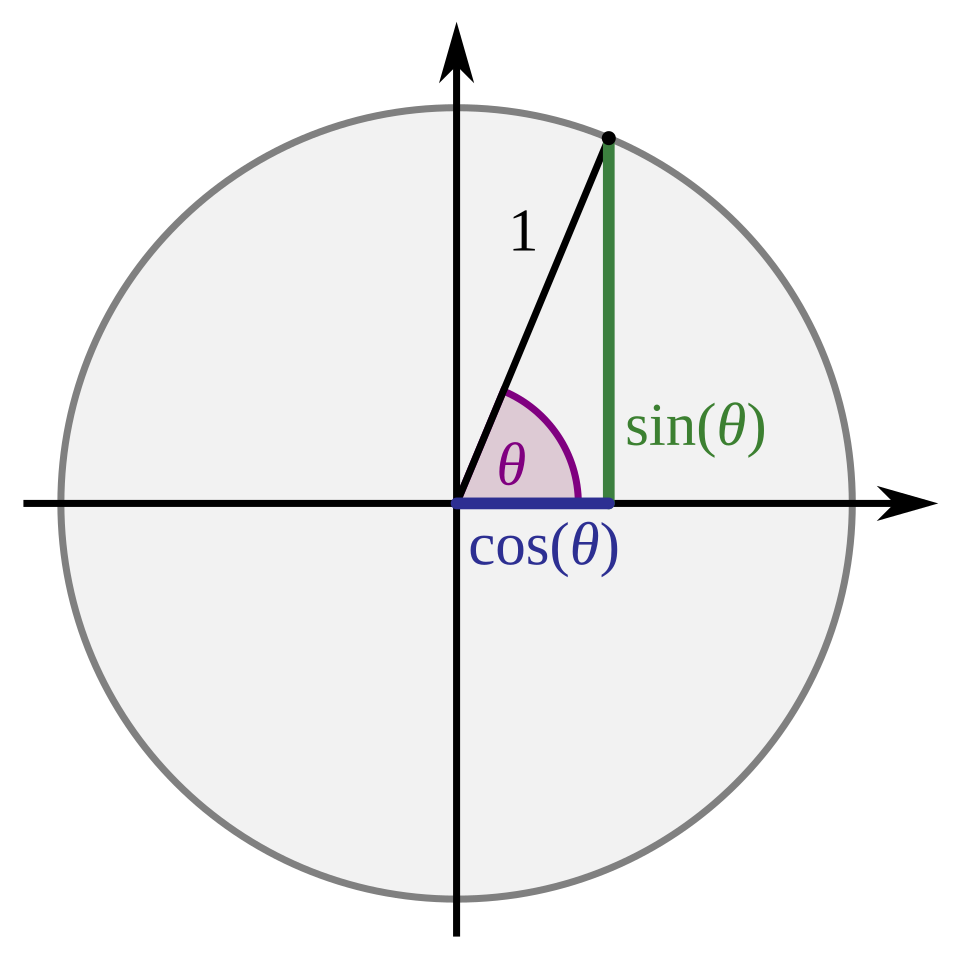
\includegraphics[height=2.5in]{sin-cos.png}


  \vfill
  \hrule
  \vspace{0.2em}

  \vspace{-.5em}

\begin{multicols}{3}
  \begin{center}

    $\vec{v} = \vec{v}_0 + \vec{a} t$
  
    \emph{\footnotesize ``Old Faithful''}
  
  
    $\vec{x} = \vec{x}_0 + \vec{v}_0 t + \frac{1}{2} \vec{a} t^2$
  
    \emph{\footnotesize``The Big Chalupa''}
  

    $\vec{v}^{\,2} = \vec{v}_0^{\,2}+ 2 \vec{a} \cdot 
    \left(\vec{x}-\vec{x}_0 \right)$

    \emph{\footnotesize ``Ain't Got No Time''}

  \end{center}
\end{multicols}

\vspace{-8pt}
\hrule
\vspace{1em}

\begin{minipage}{2.2in}
    \begin{center}
      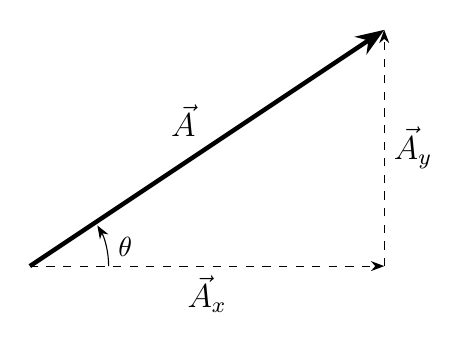
\begin{tikzpicture}[
        every node/.append style={},
        component/.append style={
          dashed,
          -{Stealth}
        },
        resultant/.append style={
          ultra thick,
          -{Stealth}
        },
    ]
      \draw[resultant] 
                (0,0) -- (4.5,3) 
                  node[midway,anchor=south east]{\large $\vec{A}$};
      \draw[component] 
                (0,0) 
                -- (4.5,0) 
                  node[midway,anchor=north]{\large $\vec{A}_x$} ;
      \draw[component] 
                (4.5,0)
                -- (4.5,3) 
                  node[midway,anchor=west]{\large $\vec{A}_y$} ;
      \draw[-Stealth] (1,0) node[anchor=south west]{$\theta$}
                arc[
                  start angle = 0,
                  end angle = 31, 
                  radius = 1
                ];
    \end{tikzpicture}


    \end{center}
  \end{minipage}
  %
  \begin{minipage}{4in}
    \begin{center}
      \begin{align*}
        A_x & = A \cos\theta &
        A_y & = A \sin\theta &
        \theta & = \tan^{-1} \left(\frac{A_y}{A_x}\right)
      \end{align*}

      \hrule 
      
      \begin{align*}
        R &= \frac{v_0^{\,2} \sin\left(2\theta\right)}{g}
      \end{align*}
      \vspace{0em}

      
    \end{center}
  \end{minipage}

  \vspace{1em}

    \hrule

  \begin{align*}
    \vec{v}_{AC} &= \vec{v}_{AB} + \vec{v}_{BC} &
    \vec{v}_{AB} &= -\vec{v}_{BA}
  \end{align*}

  \hrule


  \hrule

  \section*{Selected Answers}

  \renewcommand{\enotesize}{\normalsize}
  \renewcommand{\enoteformat}{%
    \leftskip=1.8em
    \makebox[0pt][r]{\theenmark. }%
  }

  \hfill

  \begin{multicols}{2}
    \theanswers
  \end{multicols}


\pagebreak

\hfill 

\pagebreak

\noindent
\textit{Questions and figures are from OpenStax} College Physics \textit{2nd ed (Chapter 3) or Giancolli} Physics: Principles with Applications \textit{7th ed. (Chapter 3) unless otherwise noted.}

\section*{Graphical Vector Addition}



\begin{myquestions}

\myquestion (Original problem)  \answer{$\approx 5$~km, $\approx 40^\circ$ north of east}
A hiker walks 4.0 km east and then 3.0 km north. Use a scale drawing to estimate the magnitude and direction of the hiker's displacement.

\myquestion (Original problem)  \answer{2 m east}
A robot moves 5.0 m north, 2.0 m east, and 5.0 m south. Draw the vectors tip-to-tail and determine the final displacement graphically.


\end{myquestions}

\begin{center}
  \begin{tikzpicture}
    %\draw[gray,dashed,thin] (0,0) grid (16,10);
    \draw[dotted,thin] (0,0) grid[step=0.5] (16,10);
  \end{tikzpicture} 
\end{center}

\begin{enumerate}[resume]
\myquestion (Original question)  \answer{(a) 10.0 m; (b) 2.0 m; (c) 7.21 m }
Two displacement vectors have magnitudes 6.0 m and 4.0 m. Sketch the resultant when the vectors point (a) in the same direction, (b) in opposite directions, and (c) at right angles.  Calculate the magnitude of each resultant.
\end{enumerate}


\pagebreak

\section*{Components of Vectors}







\begin{myquestions}






\myquestion (OpenStax P16)  Suppose you walk 18.0 m straight west and then 25.0 m straight north. How far are you from your starting point, and what is the compass direction of a line connecting your starting point to your final position?  %(If you represent the two legs of the walk as vector displacements $\vec{A}$ and $\vec{B}$, as in Figure~\ref{3-55}, then this problem asks you to find their sum $\vec{R}=\vec{A}+\vec{B}$.) 
\answer{30.8 m @ 35.8$^\circ$ W of N}

  % \begin{figure}[H]
  %   \centering
  %   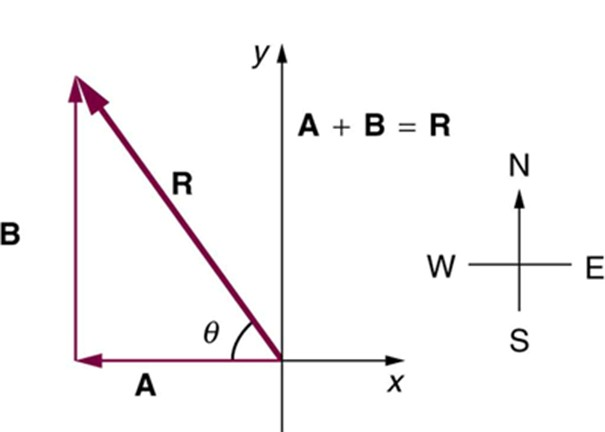
\includegraphics[width=2.2in]{3-55.jpg}
  %   \caption{(OpenStax Fig 3.55) The two displacements $\vec{A}$ and $\vec{B}$ add to give a total displacement $\vec{R}$ having magnitude $R$ and direction $\theta$.}
  %   \label{3-55}
  % \end{figure}

  

\myquestion (OpenStax P18) You drive 7.50~km in a straight line in a direction $15^\circ$ east of north. Find the distances you would have to drive straight east and then straight north to arrive at the same point. (This determination is equivalent to find the components of the displacement along the east and north directions.) \answer{$R_x = 1.94$~km; $R_y = 7.24$~km}

\myquestion (OpenStax P1, modified)
Find the total distance traveled and the magnitude and direction of the displacement for path A in Figure~\ref{3-49}. (All blocks are 120 m on a side.)

\answer{(b) 480 m; (d) $379.5$ m @ $18.4^\circ$ E of N}


\myquestion (OpenStax P2, modified) Repeat problem 1 for path B in Figure~\ref{3-49}. \answer{(b) 1200 m; (d) $379.5$ m @ $18.4^\circ$ E of N}

\myquestion (OpenStax P13, modified) Repeat problem 1 for path C in Figure~\ref{3-49}. \answer{(b) 1560 m; (d) 120 m east}


\end{myquestions}

\vfill 

\begin{figure}[H]
  \centering
  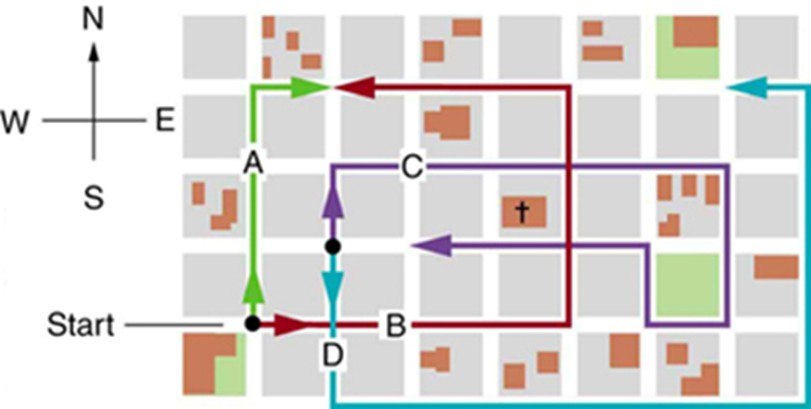
\includegraphics[height=2in]{3-49.jpg}
  \caption{(OpenStax Fig 3.49) The various lines represent paths taken by different people walking in a city. All blocks are 120 m on a side.}
  \label{3-49}
\end{figure}

\pagebreak
\section*{Vector Conceptual Questions}


\begin{enumerate}[resume]

  \myquestion (OpenStax CQ1) Which of the following is a vector: a person's height, the altitude on Mt. Everest, the age of the Earth, the boiling point of water, the cost of this book, the Earth's population, the acceleration of gravity? \vs
  \myquestion (OpenStax CQ3)  What do vectors \& scalars have in common? How do they differ? \vs
  \myquestion (Giancolli CQ1) One car travels due east at 40~km/h, and a second car traveks north at 40~km/h.  Are their velocities equal? Explain. \vs
  \myquestion (Giancolli CQ4) Can the displacement vector for a particle moving in two dimensions be longer than the length of the path traveled by the particle over the same time interval? Can it be less? Discuss. \vs
  \myquestion (OpenStax CQ9) Suppose you add two vectors $\vec{A}$ and $\vec{B}$. What relative direction between them produces the resultant with the greatest magnitude? What is the maximum magnitude? What relative direction between them produces the resultant with the smallest magnitude? What is the minimum magnitude? \vs
  \myquestion (OpenStax CQ10) Give an example of a nonzero vector that has a component of zero. \vs
  \myquestion (OpenStax CQ11) Explain why a vector cannot have a component greater than its own magnitude. \vs
  \myquestion (Giancolli CQ6) If $\vec{V}=\vec{V}_1+\vec{V}_2$, is $V$ necessarily greater than $V_1$ and/or $V_2$?  Discuss. \vs

\end{enumerate}

\pagebreak

\section*{Analytical Vector Addition}

\begin{myquestions}



\myquestion (Giancolli P6) Vector $\vec{V}_1$ is 6.6 units long and points due west.  Vector $\vec{V}_2$ is 8.5 untis long and points $55^\circ$ north of east.  (a) What are the $x$- and $y$- components of each vector?  (b) Determine the sum $\vec{V}_1+\vec{V}_2$ (magnitude and angle). \answer{$v_{1x} = -6.6$, $v_{1y} = 0$; $v_{2x} = 4.88$, $v_{2y} = 6.96$; 7.17 units @ 76.1$^\circ$ N of W}

\myquestion (Giancolli P9, P10, P12) Three vectors are shown in Figure~\ref{3-35}.  Their magnitudes are given in arbitrary units. \answer{(b) $R_x = 24.0$, $R_y = 11.7$, $\vec{R} = 26.7$ units @ 26$^\circ$ N of E; (c) 53.6 units @ 1.4$^\circ$ N of W; (d) 137.3 @ 73.0$^\circ$ W of S}

\begin{parts}
  \part Calculate the components of each vector.
  \part Draw and calculate $\vec{A}+\vec{B}+\vec{C}$ (magnitude and direction).
  \part Draw and calculate $\vec{B}-\vec{A}$ (magnitude and direction).
  \part Draw and calculate $\vec{B}-3\vec{A}$  (magnitude and direction).
\end{parts}

  \begin{figure}[H]
    \centering
    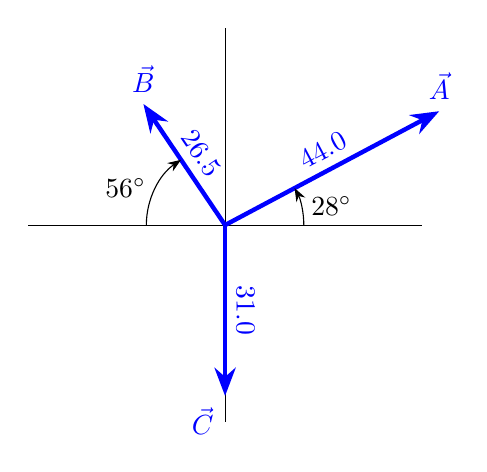
\begin{tikzpicture}
      \def\scale{0.07}
      \draw (-2.5,0) -- (2.5,0);
      \draw (0,2.5) -- (0,-2.5);
      \draw[blue, ultra thick, -Stealth] (0,0) -- (28:44*\scale) 
        node[anchor=south] {$\vec{A}$} node[midway,sloped,above] {$44.0$};
      \draw[-Stealth] (0:1) arc (0:28:1) node[midway,anchor=west] {$28^\circ$};
      \draw[blue, ultra thick, -Stealth] (0,0) -- (124:26.5*\scale)
        node[anchor=south] {$\vec{B}$} node[midway,sloped,above] {$26.5$};
      \draw[-Stealth] (-1,0) arc (180:124:1) 
        node[midway,anchor=east] {$56^\circ$};
      \draw[blue, ultra thick, -Stealth] (0,0) -- (0,-31*\scale) 
        node[anchor=north east] {$\vec{C}$} node[midway,sloped,above] {$31.0$};

    \end{tikzpicture}
    \caption{Vector magnitudes are given in arbitrary units.}
    \label{3-35}
  \end{figure}
\end{myquestions}








\pagebreak

\section*{Projectile Motion (Part I)}

\begin{myquestions}

\myquestion (Giancolli P17) \answer{3.71 m}
A tiger leaps horizontally from a 7.5-m-high rock with a speed of 3.0~m/s. How far from the base of the rock wil she land?



\myquestion (OpenStax P25) 
A projectile is launched at ground level with an initial speed of 50.0~m/s at an angle of $30.0^\circ$ above the horizontal. It strikes a target above the ground 3.00 seconds later. What are the $x$ and $y$ distances from where the projectile was launched to where it lands? \answer{$x=\SI{130}{m}$; $y=\SI{30.9}{m}$}

\myquestion (OpenStax P26)
A ball is kicked with an initial velocity of 16 m/s in the horizontal direction and 12 m/s in the vertical direction. (a) At what speed does the ball hit the ground? (b) For how long does the ball remain in the air? (c) What maximum height is attained by the ball? \answer{(a) 20 m/s; (b) 2.45 s; (c) 7.35 m}

\myquestion (OpenStax P27)
A ball is thrown horizontally from the top of a 60.0-m building and lands 100.0 m from the base of the building. Ignore air resistance. (a) How long is the ball in the air? (b) What must have been the initial horizontal component of the velocity? (c) What is the vertical component of the velocity just before the ball hits the ground? (d) What is the total velocity of the ball just before it hits the ground?
\answer{(a) 3.50 s; (b) 28.6 m/s; (c) 34.3 m/s; (d) 44.7 m/s @ 50.2$^\circ$ below horizontal}



\end{myquestions}


\pagebreak


\section*{Additional Practice}
These problems are provided for extra practice.  They are \emph{not required} and there is no bonus for doing them.
  
\begin{myquestions}
  
\myquestion   \label{SanFran} (OpenStax P15) Find the north and east components of the displacement from San Francisco to Sacramento shown in Figure~\ref{3-54}. \answer{$S_x=S_y=\SI{87.0}{km}$}

  \begin{figure}[H]
    \centering
    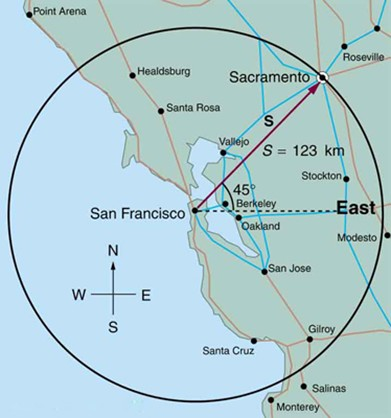
\includegraphics[width=2in]{3-54.jpg}
    \caption{(OpenStax Fig~3.54) For problem \#\ref{SanFran}.}
    \label{3-54}
  \end{figure}

\myquestion (Giancolli P3) \answer{11.7 units @ 33.1$^\circ$ S of E}
If $V_x=9.80$~ units and $V_y=-6.40$~units, determine the magnitude and direction of $\vec{V}$

\myquestion (Giancolli P10) \answer{(a) 53.6 units @ $1.4^\circ$ N of W; (b) 53.6 units @ $1.4^\circ$ S of E}
(a) Given the vectors $\vec{A}$ and $\vec{B}$ shown in Figure~\ref{3-35} on the previous page, determine $\vec{B}-\vec{A}$. (b) Determine $\vec{A}-\vec{B}$ without using your answer in (a). Then compare your results and see if they are opposite.

\myquestion (Giancolli P12) \answer{149.6 units @ $54.6^\circ$ S of E}
For the vectors shown in Figure~\ref{3-35} on the previous page, determine $2\vec{A}-3\vec{B}+2\vec{C}$.

\end{myquestions}

\hrule

\section*{Bonus}

You will be given bonus if you complete these problems \emph{on a separate sheet of paper}
  
\begin{myquestions}
  

\myquestion (OpenStax P23) \answer{7.34 km @ $63.5^\circ$ S of E}
In an attempt to escape his island, Gilligan builds a raft and sets to sea. The wind shifts a great deal during the day, and he is blown along the following straight lines: 2.50~km  $45.0^\circ$ north of west; then 4.70~km  $60.0^\circ$ south of east; then 1.30~km $25.0^\circ$ south of west; then 5.10~km  straight east; then 1.70~km  $5.00^\circ$ east of north; then 7.20~km  $55.0^\circ$ south of west; and finally 2.80~km  $10.0^\circ$ north of east. What is his final position relative to the island?

\end{myquestions}

\hrule

  
\end{document}